\documentclass[border=10pt]{standalone}
\usepackage[svgnames]{xcolor}
\usepackage{amsmath}
\usepackage{pgfplots}
\pgfplotsset{compat=newest}
\usepackage[sfdefault]{FiraSans}
\usepackage{FiraMono}
\renewcommand*\familydefault{\sfdefault}
\begin{document}
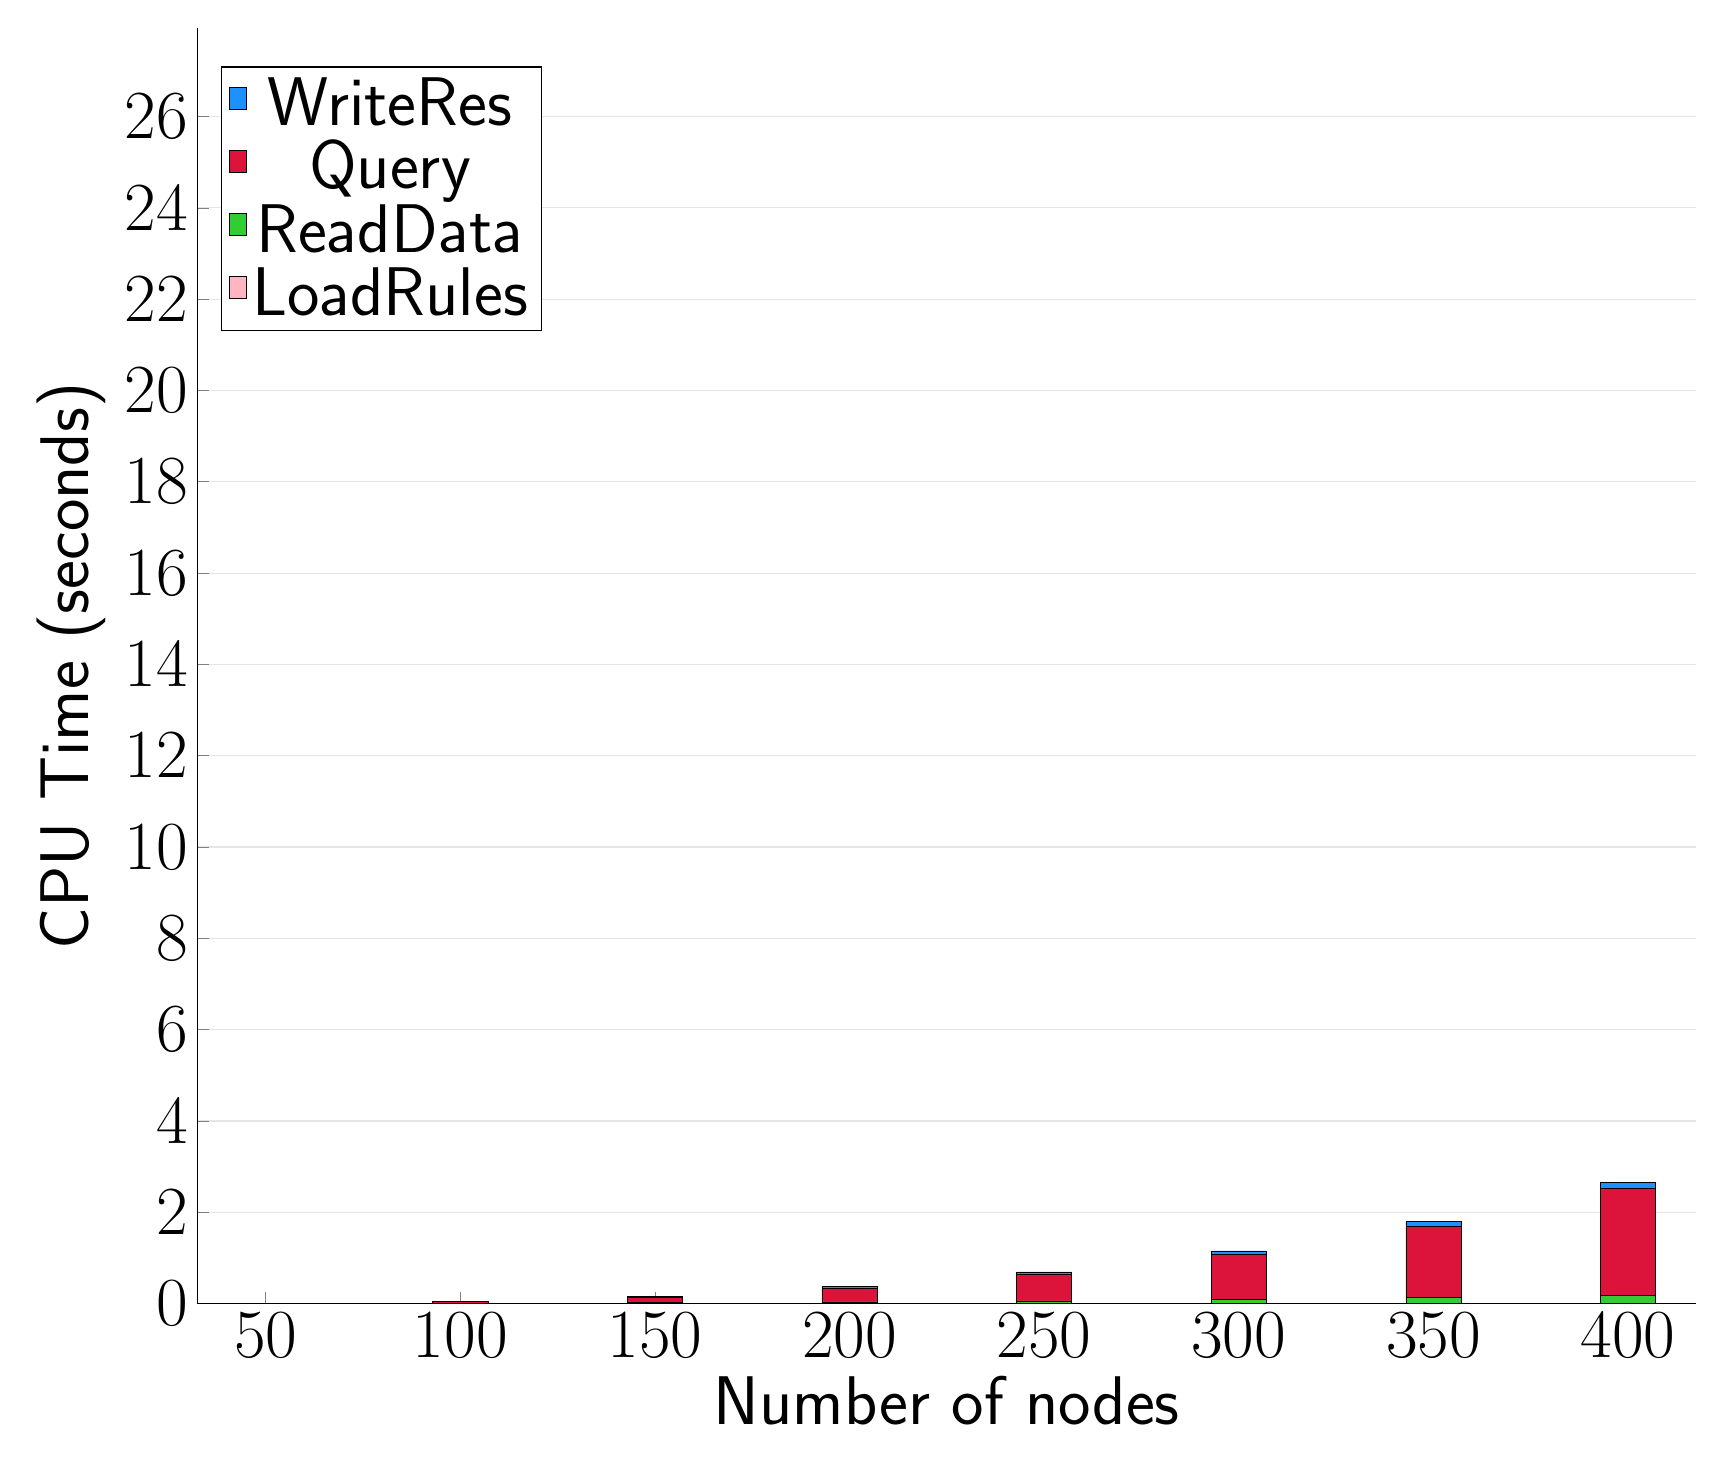
\begin{tikzpicture}
\begin{axis}[
   ybar stacked,
   width=1.7\textwidth,
   bar width=0.7cm,
   ymajorgrids, tick align=inside,
   major grid style={draw=gray!20},
   xtick=data,
   ymin=0, ymax=27.933910000000004,
   axis x line*=bottom,
   axis y line*=left,
   enlarge x limits=0.05,
   legend style={
       at={(0.23, 0.97)},
       anchor=north east,
       legend columns=1,
       font=\Huge,
   },
   ylabel={CPU Time (seconds)},
   xlabel={Number of nodes},
   label style={font=\Huge},
   tick label style={font=\Huge},
]
\addlegendimage{fill=DodgerBlue, draw=black, line width=0.2pt}
\addlegendentry{WriteRes}
\addlegendimage{fill=Crimson, draw=black, line width=0.2pt}
\addlegendentry{Query}
\addlegendimage{fill=LimeGreen, draw=black, line width=0.2pt}
\addlegendentry{ReadData}
\addlegendimage{fill=LightPink, draw=black, line width=0.2pt}
\addlegendentry{LoadRules}
\addplot +[fill=LightPink, draw=black, line width=0.2pt] coordinates {
(50, 0.0006088999999999997)
(100, 0.0005952999999999997)
(150, 0.0005922000000000004)
(200, 0.0006127999999999998)
(250, 0.0006257000000000001)
(300, 0.0006165999999999998)
(350, 0.0006244999999999998)
(400, 0.0006453000000000001)
};
\addplot +[fill=LimeGreen, draw=black, line width=0.2pt] coordinates {
(50, 0.0022530000000000002)
(100, 0.008904299999999999)
(150, 0.0207792)
(200, 0.038480099999999996)
(250, 0.06126210000000001)
(300, 0.0909852)
(350, 0.1278388)
(400, 0.1712944)
};
\addplot +[fill=Crimson, draw=black, line width=0.2pt] coordinates {
(50, 0.0045045)
(100, 0.035778700000000004)
(150, 0.12264720000000003)
(200, 0.29655529999999997)
(250, 0.5789665)
(300, 0.9814788000000002)
(350, 1.5632397999999998)
(400, 2.3444772)
};
\addplot +[fill=DodgerBlue, draw=black, line width=0.2pt] coordinates {
(50, 0.0023659999999999996)
(100, 0.009541200000000003)
(150, 0.020965499999999998)
(200, 0.03552209999999999)
(250, 0.056446799999999984)
(300, 0.07943920000000002)
(350, 0.10904200000000001)
(400, 0.1441681)
};
\end{axis}
\end{tikzpicture}

\end{document}
